\subsubsection{Overlap weights}

As a final check, we estimate overlap weights, proposed by \cite{li2018balancing}, to estimate the overlap average treatment effect (ATO). We believe that this effect may be more similar to the ETC than the ETT, particularly because there were no Democratic controlled states that did not expand Medicaid; we therefore expect this region will be far more Republican than the non-expansion region. However, it is unclear how the pre-treatment outcomes will compare relative to either the non-expansion or expansion region, which may also be an important effect modifier. Regardless, all weights are positive so that we do not have to extrapolate beyond the support of the data to obtain an unbiased estimate of this treatment effect under our modeling assumptions. 

Specifically, we regress treatment assignment on all covariates using logistic regression; letting $\hat{\pi} = \hat{\pi}(\hat{eta}(W_{sc}))$ be the predicted probabilities from the model, we then set CPUMA-level weights $\gamma_{sc} = A_{sc}(1 - \hat{\pi}_{sc}) + (1 - A_{sc})\hat{\pi}_{sc}$, where $\hat{\pi} = \hat{\pi}(\hat{\eta}(W_{sc}))$.\footnote{Since treatment assignment is at the state-levels, these are not propensity scores. We instead use these scores for their covariate balancing properties.} As discussed in \cite{li2018balancing}, these weights exactly balance the mean of the control region to the treated region:

\begin{equation}
    \frac{\sum_{s, c: A_s = 1} \gamma_{sc}\hat{\eta}_1(W_{r, sc})}{\sum_{s, c: A_s = 1}\gamma_{sc}} = \frac{\sum_{s, c: A_s = 1}\gamma_{sc}\hat{\eta}_0(W_{r, sc})}{\sum_{s, c: A_s = 0}\gamma_{sc}} \ \ \ (r = 1, ..., q)
\end{equation}

We then estimate the ATO as

\begin{equation}
    \psi^{ATO} = \frac{\sum_{s, c: A_s = 1} \gamma_{sc}J_{sc}}{\sum_{s, c: A_s = 1}\gamma_{sc}} - \frac{\sum_{s, c: A_s = 1}\gamma_{sc}J_{sc})}{\sum_{s, c: A_s = 0}\gamma_{sc}}
\end{equation}


\subsubsection{Covariate overlap}

To this point we have relied on either (1) retaining a potentially biased estimate from weights that do not exactly balance the covariates, or (2) relying on more model-dependent estimates via extrapolation. Overall we found that the results did not change substantially either way. We now consider instead the overlap average treatment effect (ATO), as discussed above. After generating overlap weights on our primary dataset we find that across all covariates, the mean average absolute distance from the overlap region to the untreated region is 2.24 and to the treated region is 7.55. \footnote{This distance is calculated on the adjusted dataset. When excluding early expansion states the mean L1 distance is 2.21 to the untreated and 5.19 to the treated region.} Figure~\ref{fig:ATOimbalance} displays the distance between covariates with greater than one percentage point distance from the overlap region to either the control or treated region. We see that the overlap region is substantially more Republican than the treated region. If our research hypothesis is correct, this should indicate that the ATO will be closer to the ETC than the ETT. This region is also less Hispanic, more white, and more educated than either the expansion or non-expansion region. Interestingly, it also has lower pre-treatment uninsurance rates than either the treated or untreated regions. Table~\ref{tab:ATOdist1} in Appendix D shows additional statistics on the ATO region versus the treatment and control regions for all covariates.

\begin{figure}[H]
\begin{center}
    \caption{Overlap area compared to treated, untreated regions}
    \label{fig:ATOimbalance}
    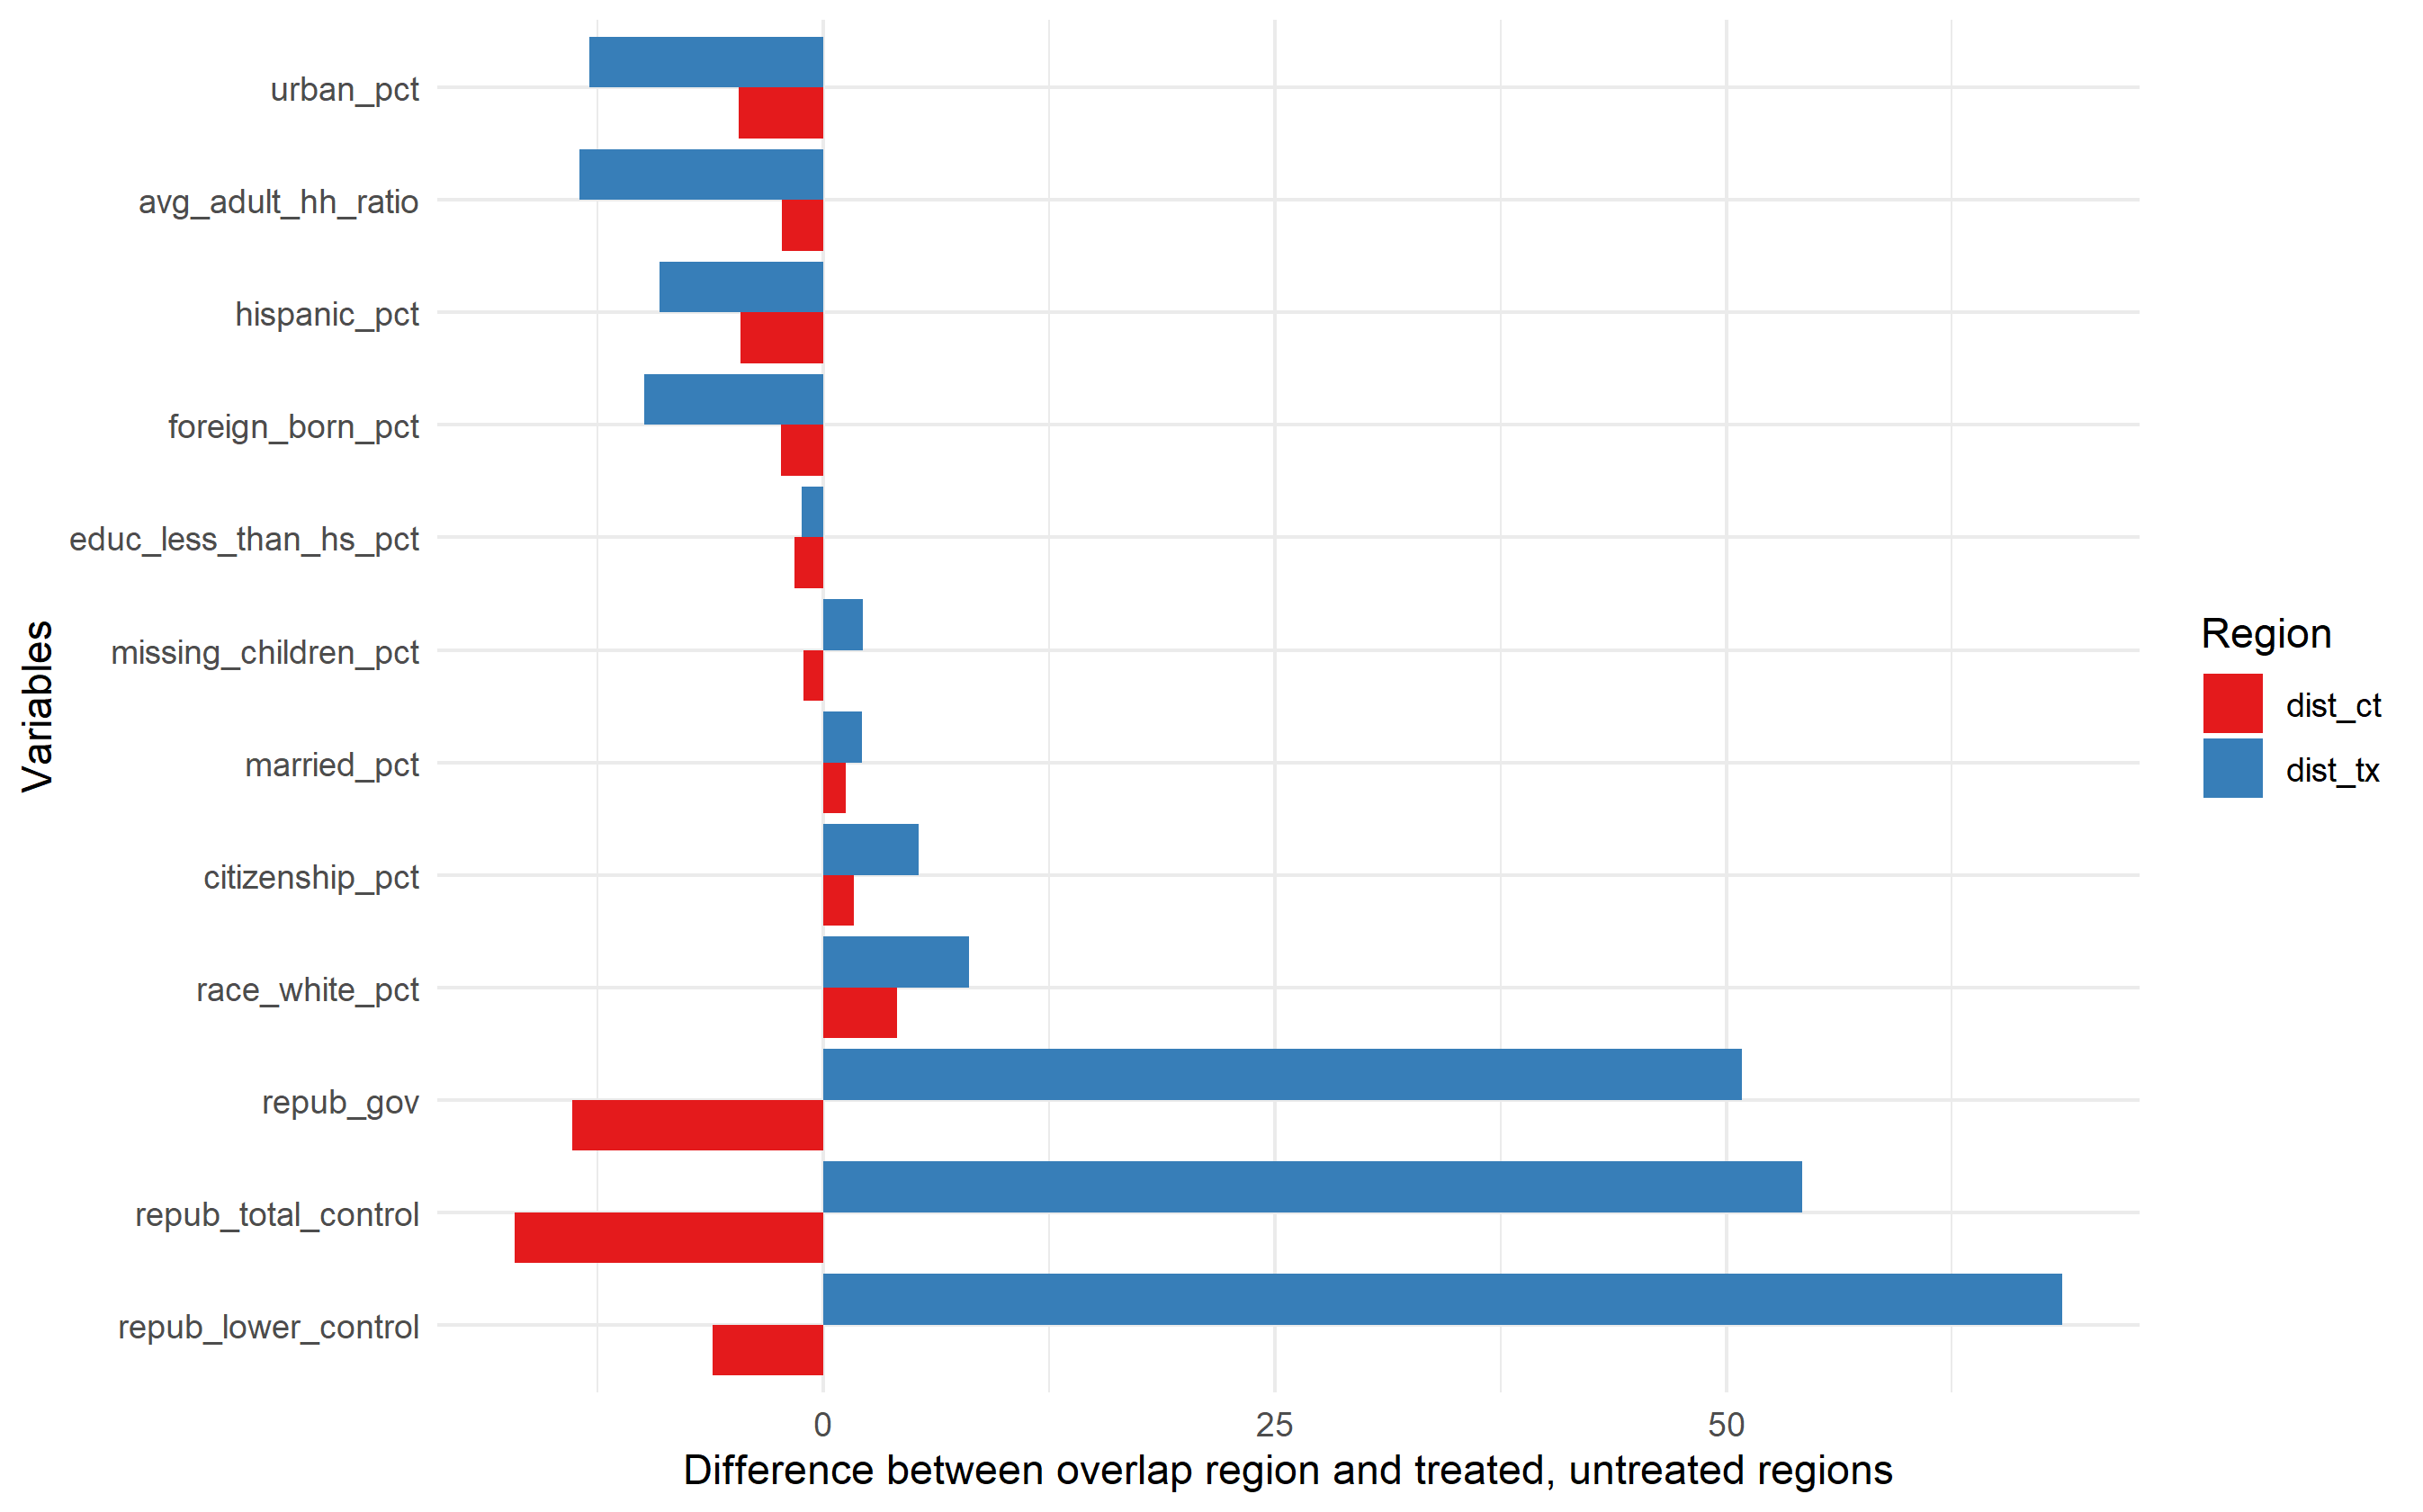
\includegraphics[scale=0.6]{01_plots/oate-imbalances-c1.png}
\end{center}
\end{figure}

Figure~\ref{fig:ATOimbalance} displays the sum of the weights within each state by treatment group. Ohio, Michigan, and Arkansas are the most heavily weighted states, and all come from the expansion region (the weights are standardized within each treatment group to sum to 100). The weights are more evenly dispersed among the non-expansion regions, though Pennsylvania, Missouri, Wisconsin, and Florida are given the most weight. We note that this region is specific to the preferred covariate adjustment; the results are quite similar for the unadjusted and secondary covariate adjustment and are available in Appendix D, Table ~\ref{tab:ATOstateweightsc1}.

\begin{figure}[H]
\begin{center}
    \caption{Overlap weights by state}
    \label{ATOarea}
    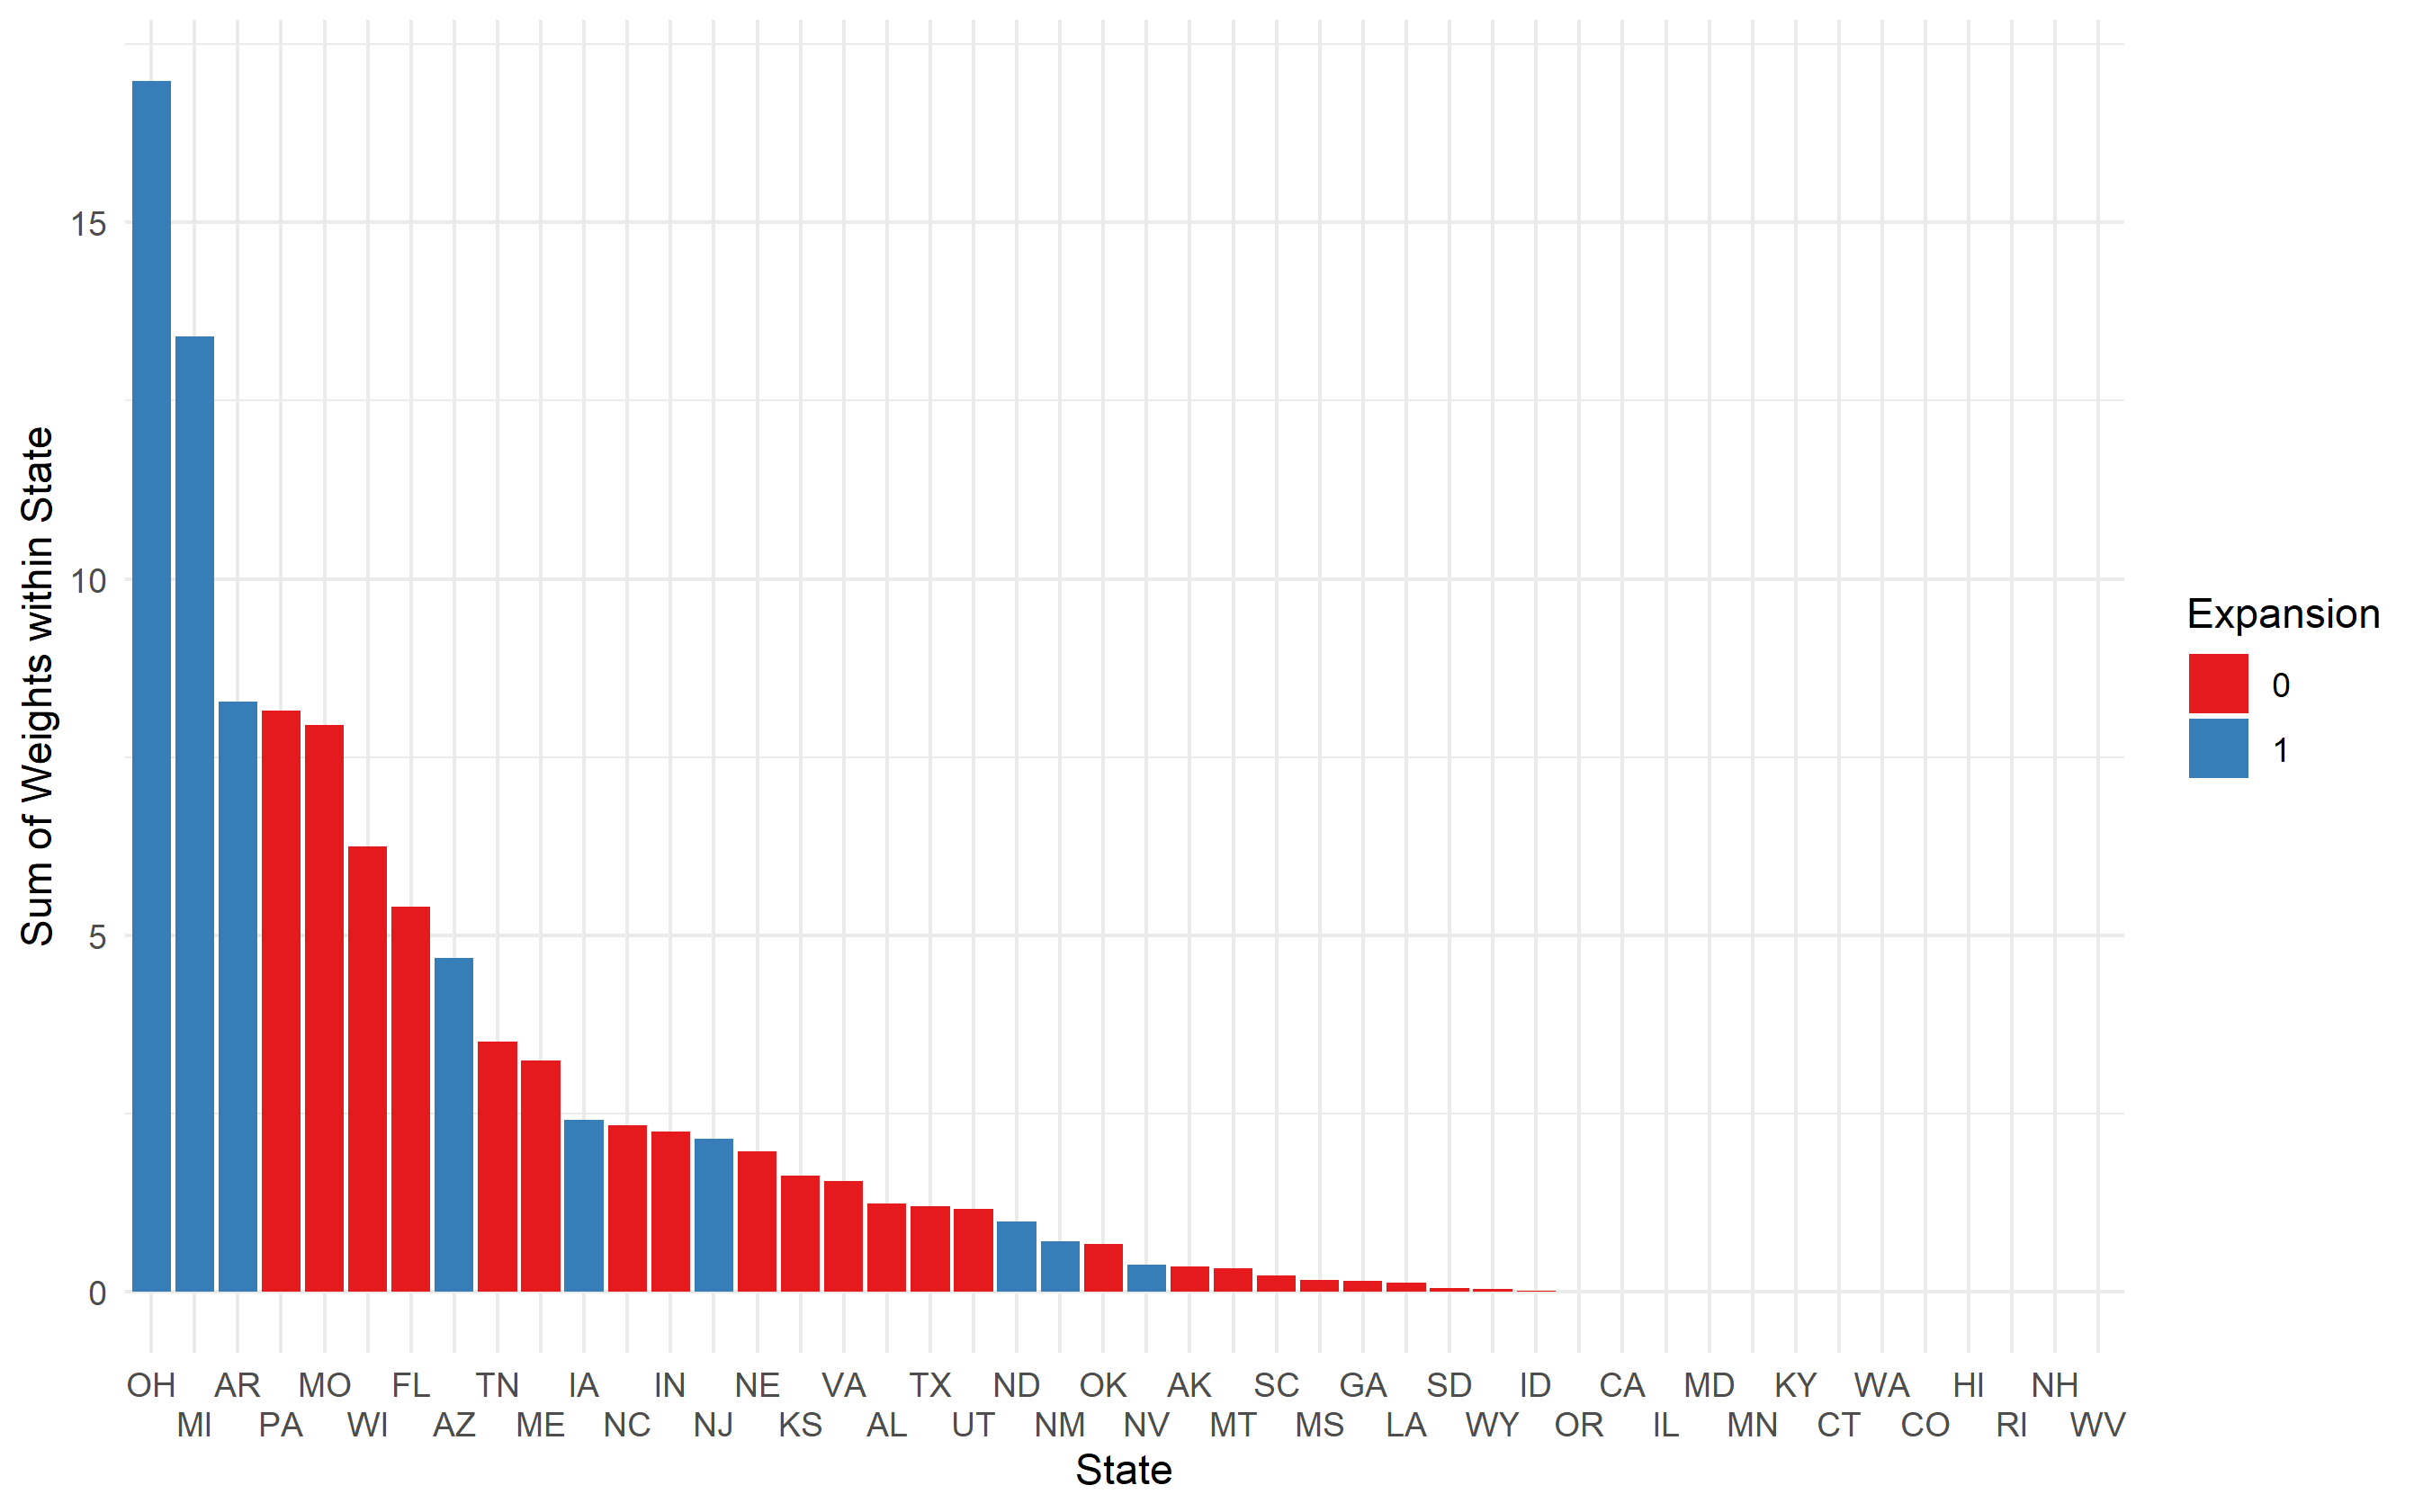
\includegraphics[scale=0.6]{01_plots/oate-region-c1-a.png}
\end{center}
\end{figure}

The point estimates are somewhat larger relative to our primary analysis: within the overlap region we estimate a treatment effect -1.74 (-2.35, -1.14) when including all treatment states in our primary analysis, and of -1.89 (-2.47, -1.32) when excluding the early expansion states. These results are quite similar compared to the unadjusted datasets: -1.80 (-2.50, -1.10) on the primary dataset and -1.95 (-2.65, -1.25) when excluding early expansion states. These confidence intervals are much narrower than our previous estimates. This is not entirely surprising: as \cite{li2018balancing} note, the ATO has the minimum conditional variance of any weighted average treatment effect under homoskedastic errors. \footnote{The ATO weights are also not optimized for the hierarchical data structure, but rather are output from a standard logistic regression model. It would be simple to rerun the H-SBW procedure targeting the overlap weight region to generate a set of balancing weights with possibly improved properties for this data structure, though we do not do this.}

